\documentclass{beamer}
\usepackage[utf8]{inputenc}
\usetheme{Madrid}
\usecolortheme{default}
\usepackage{amsmath,amssymb,amsfonts,amsthm}
\usepackage{txfonts}
\usepackage{tkz-euclide}
\usepackage{listings}
\usepackage{adjustbox}
\usepackage{array}
\usepackage{tabularx}
\usepackage{gvv}
\usepackage{lmodern}
\usepackage{circuitikz}
\usepackage{tikz}
\usepackage{graphicx}
\setbeamertemplate{page number in head/foot}[totalframenumber]
\usepackage{tcolorbox}
\tcbuselibrary{minted,breakable,xparse,skins}
\definecolor{bg}{gray}{0.95}
\DeclareTCBListing{mintedbox}{O{}m!O{}}{%
  breakable=true,
  listing engine=minted,
  listing only,
  minted language=#2,
  minted style=default,
  minted options={%
    linenos,
    gobble=0,
    breaklines=true,
    breakafter=,,
    fontsize=\small,
    numbersep=8pt,
    #1},
  boxsep=0pt,
  left skip=0pt,
  right skip=0pt,
  left=25pt,
  right=0pt,
  top=3pt,
  bottom=3pt,
  arc=5pt,
  leftrule=0pt,
  rightrule=0pt,
  bottomrule=2pt,
  toprule=2pt,
  colback=bg,
  colframe=orange!70,
  enhanced,
  overlay={%
    \begin{tcbclipinterior}
    \fill[orange!20!white] (frame.south west) rectangle ([xshift=20pt]frame.north west);
    \end{tcbclipinterior}},
  #3,
}
\lstset{
    language=C,
    basicstyle=\ttfamily\small,
    keywordstyle=\color{blue},
    stringstyle=\color{orange},
    commentstyle=\color{green!60!black},
    numbers=left,
    numberstyle=\tiny\color{gray},
    breaklines=true,
    showstringspaces=false,
}
\begin{document}

\title 
{10.7.4}
\date{september 14,2025}


\author 
{Namaswi-EE25BTECH11060}
\frame{\titlepage}
\begin{frame}{Question}
    Prove that $y=2x+2\sqrt{3}$  is commom tangent to the parabola $y^2=16\sqrt{3}x$ and the ellipse $2x^2+y^2=4$
\end{frame}
\begin{frame}{Solution}
    General Formulae of a conic\\
\begin{align}
\vec{x}^T V \vec{x} + 2 \vec{u}^T \vec{x} + f = 0
\end{align}
The tangent condition for line $\vec{n}^T \vec{x} + c = 0$ at contact point $\vec{q}$ is
\begin{align}
V\vec{q} + \vec{u} = \lambda \vec{n}\\ 
\vec{u}^T \vec{q} + f = \lambda c
\end{align}
\end{frame}
\begin{frame}{Solution}
for some scalar $\lambda$.
For Parabola $y^2 = 16\sqrt{3}\,x$
 \begin{align}
V = \begin{pmatrix}0 & 0 \\ 0 & 1\end{pmatrix}\\
\quad 
\vec{u} = \begin{pmatrix}-8\sqrt{3} \\ 0\end{pmatrix}\\
\quad 
f = 0.
\end{align}

Line: $2x - y + 2\sqrt{3} = 0$, so
\begin{align}
\vec{n} = \begin{pmatrix}2 \\ -1\end{pmatrix} \\
\quad c = 2\sqrt{3}
\end{align} 
\end{frame}
\begin{frame}{Solution}
\noindent First condition
\begin{align}
V\vec{q} + \vec{u} = \begin{pmatrix}-8\sqrt{3} \\ y\end{pmatrix} 
= \lambda \begin{pmatrix}2 \\ -1\end{pmatrix}.
\end{align}
Thus $\lambda = -4\sqrt{3}$  and $y = 4\sqrt{3}$.

\noindent Second condition:
\begin{align}
\vec{u}^T \vec{q} + f = -8\sqrt{3}\,x = \lambda c = (-4\sqrt{3})(2\sqrt{3}) = -24,
\end{align}
giving $x = \sqrt{3}$. 
\end{frame}
\begin{frame}{Solution}
\begin{align}
{\vec{q} = \begin{pmatrix}\sqrt{3} \\ 4\sqrt{3}\end{pmatrix}}
\end{align}

So the line touches the parabola at $(\sqrt{3}, 4\sqrt{3})$.

For Circle $2x^2 + y^2 = 4$
\begin{align}
V = \begin{pmatrix}2 & 0 \\ 0 & 1\end{pmatrix}\\
\quad 
\vec{u} = \begin{pmatrix}0 \\ 0\end{pmatrix}\\
\quad 
f = -4.
\end{align}   
\end{frame}
\begin{frame}{Solution}
\noindent First condition:
\begin{align}
V\vec{q} = \lambda \vec{n}
\end{align}
we get 
\begin{align}
\vec{q} = \lambda \begin{pmatrix}1 \\ -1\end{pmatrix}.
\end{align}

\noindent Second condition:
\begin{align}
\vec{u}^T\vec{q} + f = -4 = \lambda c = \lambda(2\sqrt{3})
\quad \\ \Rightarrow \quad \lambda = -\frac{2}{\sqrt{3}}.
\end{align}
\end{frame}
\begin{frame}{Solution}
So
\begin{align}
\vec{q} = -\frac{2}{\sqrt{3}} \begin{pmatrix}1 \\ -1\end{pmatrix}
= \begin{pmatrix}-\tfrac{2\sqrt{3}}{3} \\ \tfrac{2\sqrt{3}}{3}\end{pmatrix}.
\end{align}
\begin{align}
{\vec{q} = \begin{pmatrix}-\tfrac{2\sqrt{3}}{3} \\ \tfrac{2\sqrt{3}}{3}\end{pmatrix}}
\end{align}
So the line touches the circle at $\left(-\tfrac{2\sqrt{3}}{3}, \tfrac{2\sqrt{3}}{3}\right)$.
Hence given line is common tangent to both the curves.    
\end{frame}
\begin{frame}[fragile]
\frametitle{Python Code}
\begin{lstlisting}
    import numpy as np
import matplotlib.pyplot as plt
# Line: y = 2x + 2√3
def line(x):
    return 2*x + 2*np.sqrt(3)
# Parabola: y^2 = 16√3 x => x = y^2 / (16√3)
y_parabola = np.linspace(-10, 10, 400)
x_parabola = y_parabola**2 / (16 * np.sqrt(3))
# Ellipse: 2x^2 + y^2 = 4
theta = np.linspace(0, 2*np.pi, 400)
a = np.sqrt(2)  # semi-major axis
b = 2          # semi-minor axis
\end{lstlisting}
\end{frame}
\begin{frame}[fragile]
\frametitle{Python Code}
\begin{lstlisting}
    x_ellipse = a * np.cos(theta)
y_ellipse = b * np.sin(theta)
# Line domain (chosen to cover range of ellipse and parabola)
x_line = np.linspace(-2, 2, 400)
y_line = line(x_line)

# Plotting
plt.figure(figsize=(8, 8))
plt.plot(x_parabola, y_parabola, label=r'$y^2 = 16\sqrt{3}x$', color='green')
plt.plot(x_parabola, -y_parabola, color='green')  # the other half of the parabola
\end{lstlisting}
\end{frame}
\begin{frame}[fragile]
\frametitle{Python Code}
\begin{lstlisting}
    plt.plot(x_ellipse, y_ellipse, label=r'$2x^2 + y^2 = 4$', color='blue')
plt.plot(x_line, y_line, label=r'$y = 2x + 2\sqrt{3}$', color='red', linestyle='--')

plt.axhline(0, color='black', linewidth=0.5)
plt.axvline(0, color='black', linewidth=0.5)
plt.grid(True)
plt.legend()
\end{lstlisting}
\end{frame}
\begin{frame}[fragile]
\frametitle{Python Code}
\begin{lstlisting}
    plt.title("Common Tangent to a Parabola and an Ellipse")
plt.xlabel("x-axis")
plt.ylabel("y-axis")
plt.axis('equal')
plt.show()
\end{lstlisting}
\end{frame}
\begin{frame}[fragile]
\frametitle{C Code}
\begin{lstlisting}
   #include <stdio.h>
#include <math.h>

// Define square root of 3
#define SQRT3 1.73205080757

// Function to check if a line is tangent to a conic
int check_tangent() {
    double A, B, C, D;
    double discriminant; 
\end{lstlisting}
\end{frame}
\begin{frame}[fragile]
\frametitle{ C Code}
\begin{lstlisting}
     // For Parabola: y = 2x + 2√3 into y^2 = 16√3 x
    A = 1;
    B = -2 * SQRT3;
    C = 3;
    discriminant = B*B - 4*A*C;

    if (fabs(discriminant) > 1e-6) return 0; // Not a tangent to parabola
\end{lstlisting}
\end{frame}
\begin{frame}[fragile]
\frametitle{ C Code}
\begin{lstlisting}
     // For Ellipse: y = 2x + 2√3 into 2x^2 + y^2 = 4
    A = 6;
    B = 8 * SQRT3;
    C = 8;
    discriminant = B*B - 4*A*C;

    if (fabs(discriminant) > 1e-6) return 0; // Not a tangent to ellipse

    return 1; // Common tangent
}
\end{lstlisting}
\end{frame}
\begin{frame}[fragile]
\frametitle{ Python and C Code}
\begin{lstlisting}
    import ctypes
# Load the shared object file
conic = ctypes.CDLL("./conic_tangent.so")
# Call the function
result = conic.check_tangent()
if result == 1:
    print("The line is a common tangent to both the parabola and the ellipse.")
else:
    print("The line is NOT a common tangent.")
\end{lstlisting}
\end{frame}
\begin{frame}{plot}
\centering
    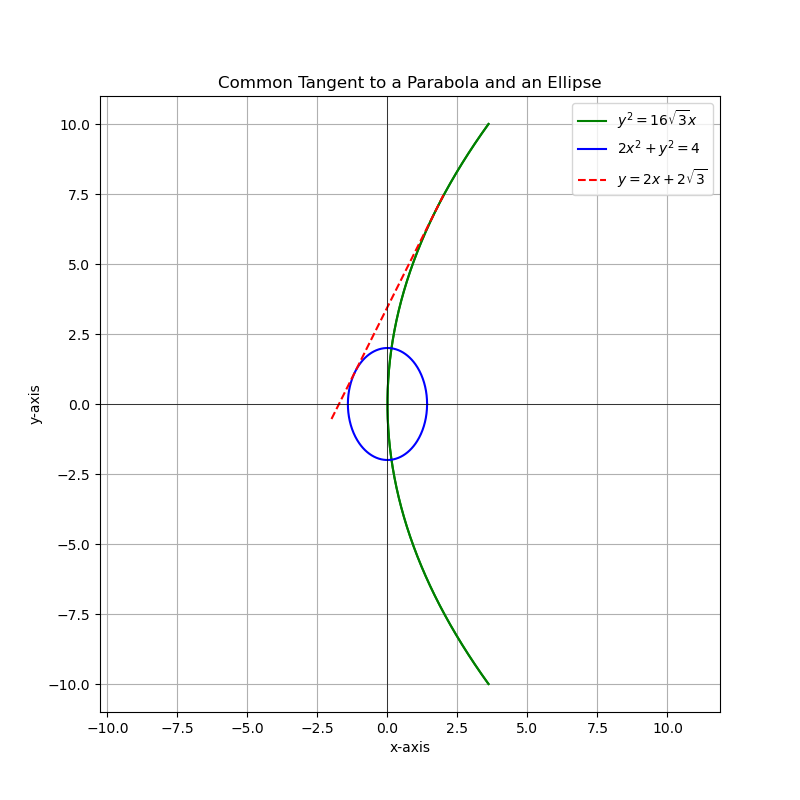
\includegraphics[width=\columnwidth, height=0.8\textheight, keepaspectratio]{Figure_17.png}
   
\end{frame}
\end{document}